\renewcommand{\leftmark}{NOMINATION DES TECHNOLOGIES}

\chapter{Rappels et nomination des technologies}

\section{Signal radio}

Un signal est une variation dans l'espace ou dans le temps d'une quantité physique contenant de l'information. Un signal peut être continu ou discret, on le nomme alors respectivement analogique ou numérique. Le type de signal dépent notamment de l'information qu'il contient. Un signal analogique peut contenir par exemple du son, là où un signal numérique contient généralement un nombre fini de valeur (par exemple des 0 et 1).
Les deux catégories ne sont pas incompatible car il est souvent nécessaire en télécommication de pouvoir passer de l'un à l'autre.

\vspace{0.1cm}

L'utilisation de signaux radio en télécomunication confère de nombreux avantages, comme la portée, la vitesse de transmission , la résistance aux interférence ou encore le coût de propagation. Tout ces avantages sont possibles car un signal peut être modulé. La modulation est une technique permettant de modifier les propriétés du signal lui permettant de transporter de l'information.

\newpage

En télécommunication, les signaux sont associés aux ondes radios, ainsi appelé $radio$ $signal$ ou signal radio. Voici les principaux attributs d'un signal radio: 

\vspace{0.1cm}

\begin{itemize}

\item la fréquence, mesurée en Hertz ($Hz$). Elle détermine le nombre de cycle qu'accomplie le signal par seconde.
\item La largeur de spectre, elle dépent de la fréquence car c'est l'écart entre la plus haute et la plus basse fréquence du signal. Une plus grande largeur permet de transmettre plus d'informations.
\item L'amplitude. Selon le type de signal l'attribut possède différentes fonctions. Dans le cas d'un signal analogique l'amplitude est l'une des caractéristiques principales d'identification du signal mesurant l'ampleur du signal. Dans un signal numérique l'amplitude sert plutot de marge entre les différentes états du signal. 
\item la puissance, mesurée en Décibel ($dB$). C'est la force du signal, un attribut important pour la réception du signal notamment.
\item le $signal$ $to$ $noise$ $ratio$ ou $SNR$. Cet attribut mesure la qualité du du signal. une valeur élevée indique que le pourcentage de bruit est faible.
\item le $bit$ $rate$, ou le taux de transmission mesure la quantité de donnée transmise en bit par seconde. Cet attribut est exclusif aux signaux numériques. On parle de $Baud$ $rate$ pour les signaux analogiques. Ce n'est pas excatement l'équivalent du bit rate car c'est le nombre de symboles modifiés par seconde, et un symbole peut contenir plusieurs bit pour un signal numérique.

\end{itemize}

\section{Traitement du signal}

\subsubsection{Modulation}

La réception d'un signal nécessite des antennes dont les dimensions dépendent de la longueur d'onde du signal. Un signal à haute fréquence a l'avantage d'être facilement transmissible sur une grand portée. Cependant les signaux originaux (appelés $baseband$ $signals$) sont en basse fréquence. La modulation d'un signal permet de transformer le signal en haute fréquence, devenant ainsi le signal modulé.

\vspace{0.1cm}

Parmis ces différents attributs, certains sont utilisés pour effectuer une modulation. Les deux modulations les plus utilisés sont basées sur les attributs de la fréquence et de l'amplitude. La modulation en fréquence (ou $FM$ pour $frequency$ $modulation$) consiste à encoder l'information en faisant varier la fréquence en maitenant l'amplitude constante. La modulation en amplitude ($AM$) est le procédé inverse, c'est à dire encoder l'information en faisant varier l'amplitude tout en gardant la fréquence constante. 

\vspace{0.1cm}

La modulation en amplitude est plus ancienne et est encore utilisée dans beaucoup de systèmes. Cette technique possède moins de contrainte et est notamment plus simple à implémenter. Elle requiert le signal modulant et un signal haute fréquence appelé $carrier$ $signal$.

\vspace{0.1cm}

Soient un signal modulant $u(t)$ et un sigal porteur (ou $carrier$ $signal$) $v(t)$, la modulation en amplitude s'effectue en multipliant les deux signaux pour obtenir le signal modulé 

\vspace{0.1cm}

$s(t)$ = $u(t)$ . $v(t)$

\begin{figure}[h]
\centering

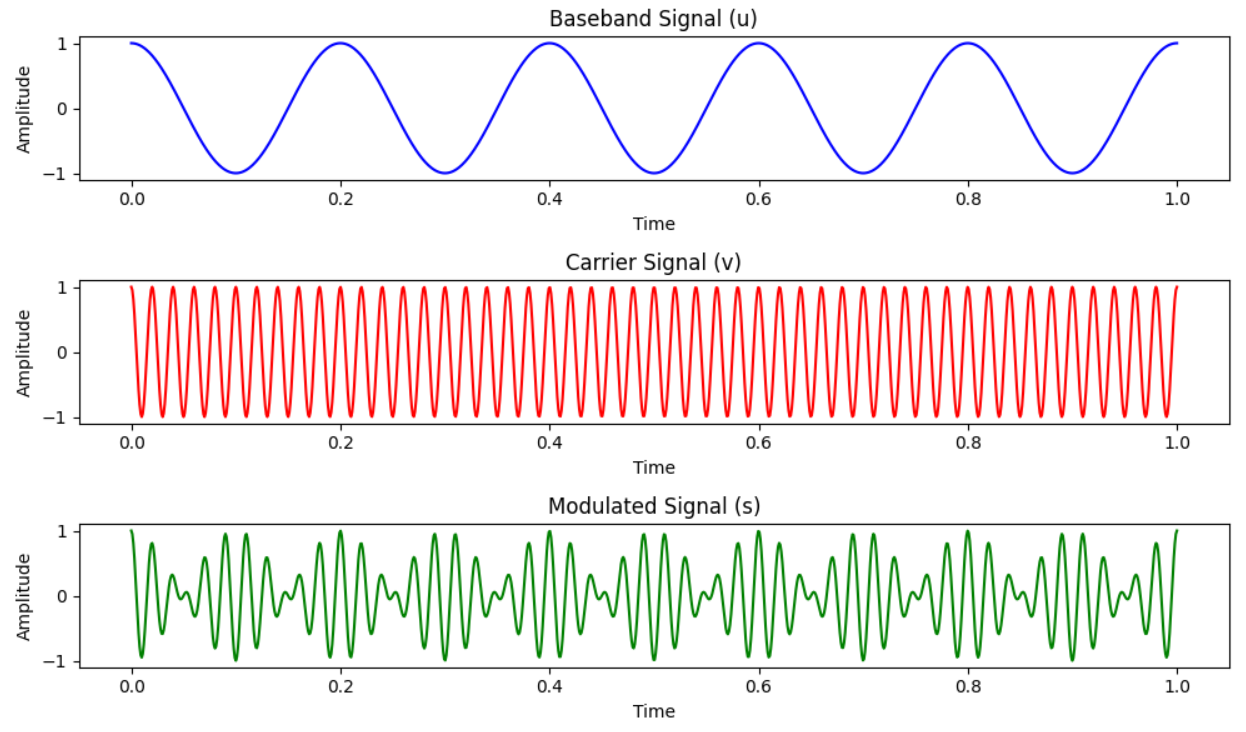
\includegraphics[scale=1]{../images/AM_mod.PNG}
\caption{Exemple de modulation en amplitude}\label{term4}
\end{figure}


La modulation en fréquence permet d'obtenir des transmissions de meilleures qualités plus résistantes à leur environement tout en gardent une puissance d'émission constante. 

\vspace{0.1cm}

Soient un signal modulant $u(t)$ et un signal porteur sinuosidal

\vspace{0.1cm}

$v_{p}(t)$ = $A_{p}cos(2\pi f_{p}t)$ où

$f_{p}$ est la fréquence de la porteuse,

$A_{p}$ est l'amplitude de la porteuse,

alors le signal modulé $s(t)$ = $A_{p}cos(2\pi \int_{0}^{t}f(\tau)d\tau)$ où $f$ est la fréquence instantanée. Elle s'exprime en fonction de la dérivation de fréquence $f_{\Delta}$, c'est à dire la dérivation maximale par rapport à la fréquence de la porteuse.

\newpage

$f_{p}$. $f(t)$ = $f_{p}$ + $f_{\Delta} u(t)$

\begin{figure}[h]
\centering

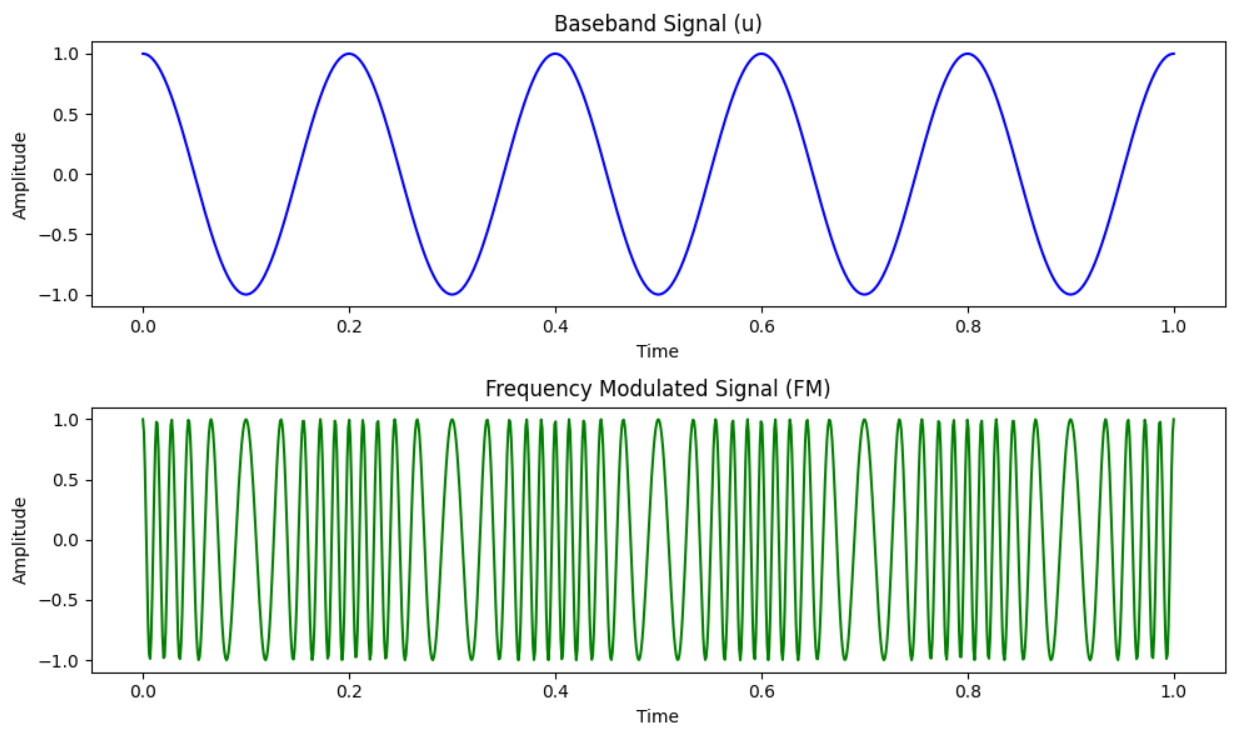
\includegraphics[scale=1]{../images/FM_mod.PNG}
\caption{Exemple de modulation en fréquence}\label{term4}
\end{figure}



\subsubsection{Gestion du bruit}



L'un des attributs cités concerne le bruit. Un signal est toujours affecté de petites fluctuations plus ou moins importantes, et dont les origines peuvent être diverses. Ces perturbations, appelée bruit ou $noise$ en télécommunication se définissent par l'altération non souhaitée de l'intégrité d'un signal. Le bruit peut prendre différentes formes, des perturbations essentiellement impulsionnelles engendrées par des commutations de courants ou alors du bruit de fond généré dans les câbles et les composants électroniques en raison
des mécanismes statistiques de la conduction électrique. Il est possible de réduire voir élimier l'influence des perturbations impulsionelles. En revanche, le bruit de fond est lui irreductible. Tout signal sans bruit n'existe pas, même à l'émission. Il est cependant possible que le bruit devienne invisible si son niveau est très faible. L'attribut SNR est donc un critère de la qualité du signal.

\newpage

\subsubsection{transformée de Fourier}

Pour effectuer une analyse de signal, sa représentation est capitale. Les Figure 1 et 2 représentent des signaux en fonction du temps écoulé. Il est possible de représenter des signaux selon une autre composante, la fréquence par exemple.

\vspace{0.1cm}

La transformée de Fourier est un outil fondamental utilisé pour analyser et décomposer des signaux complexes en composantes fréquentielles. En transformant un signal dans le domaine temporel en sa représentation dans le domaine fréquentiel, la transformée de Fourier révèle les différentes composantes fréquentielles présentes dans le signal. En fonction du type de signal, la transformée de Fourier est adaptée.

\vspace{0.1cm}

Pour les signaux continus, la $CFT$ (Transformée de Fourier continue) convertit une fonction du temps en fonction de la fréquence en intégrant le signal par rapport aux sinusoïdes de toutes les fréquences possibles. Cette transformation fournit les informations d'amplitude et de phase pour chaque composante de fréquence présente dans le signal.

\vspace{0.1cm}

Pour les signaux discrets et échantillonnés, la $DFT$ (Transformée de Fourier discrète) calcule un ensemble fini de composantes de fréquence. Il est calculé à l’aide d’un nombre fini d’échantillons, ce qui donne des composantes de fréquence discrètes. Il existe un méthode simplifiée pour les signaux discrets appelé $FFT$ (Fast Fourier Transform). Il s'agit d'un moyen plus rapide de calculer la transformée de Fourier, en particulier pour les signaux numériques comportant un grand nombre de points de données. L'avantage principal de cet algorithme permet de réduire le temps de calcul en divisant la DFT en sous problèmes. La FFT est une méthode très utilisée pour l'analyse de signaux.

\newpage

\section{LoRa}

$LoRa$ (Long Range) est une technologie de communication sans fil qui permet de transmettre des données sur de longues distances avec une faible consommation d'énergie. Elle a été développée par la société française Cycleo et est maintenant gérée par la fondation LoRa Alliance, qui regroupe plusieurs entreprises et organisations du monde entier.

\vspace{0.1cm}

LoRa est principalement utilisée dans l'$Iot$. Elle se distingue par sa portée étendue, qui peut atteindre plusieurs kilomètres en milieu urbain et plusieurs dizaines de kilomètres en milieu rural, ainsi que par sa faible consommation d'énergie, qui permet de prolonger la durée de vie des appareils connectés. Une longue portée avec un puissance limitée induit une plus faible bande passante que les autres technologies sans fil (le Wifi, la 4G, Bluetooth etc).

\vspace{0.1cm}

LoRa utilise une bande de fréquences qui varie selon les régions du monde où LoRa est déployée :

\vspace{0.1cm}

\begin{itemize}
\item en Europe, la bande de fréquences autorisée est comprise entre 863 et 870 MHz,
\item aux États-Unis, elle se situe entre 902 et 928 MHz,
\item en Chine, la fréquence autorisée varie entre 779 et 787 MHz,
\item les régions restantes ont elles aussi une fourchette unique.
\end{itemize}

\vspace{0.1cm}

La technologie LoRa utilise la modulation en fréquence chirp spread spectrum ($CSS$ $modulation$). La modulation CSS utilise un signal chirp, c'est à dire un signal modulé en fréquence linéaire. Ce signal a une amplitude constante mais balaie tout le spectre de la bande passante de manière liénaire dans une période de temps définie. Cette technique de modulation sera détaillé plus loin dans le chapitre.

\vspace{0.1cm}

La technologie LoRa utilise également une technique de multiplexage en temps partagé ($TDMA$) pour permettre à plusieurs appareils de partager la même bande de fréquences de manière à maximiser l'utilisation de la capacité de transmission. Elle utilise également une technique de diffusion de données ($multicast$) pour envoyer les mêmes données à plusieurs appareils simultanément, ce qui permet de réaliser des économies de bande passante et d'énergie.

\vspace{0.1cm}

En plus de sa portée étendue et de sa faible consommation d'énergie, LoRa se distingue par sa sécurité de transmission, qui est assurée grâce à l'utilisation de codes de sécurité uniques et à la possibilité de chiffrer les données transmises. Elle est également compatible avec de nombreux protocoles de communication couramment utilisés dans l'IoT, tels que TCP/IP, HTTP et MQTT, ce qui facilite son intégration dans les systèmes existants.

\vspace{0.1cm}

Toutes ces  particularités font de LoRa une technologie complémentaire à celles déja existente plutot que rivale.
LoRa se compose de deux éléments principaux : la couche physique de la technologie et LoRaWAN, la couche MAC ($media$ $access$ $control$), une sous couche de la couche liaison de données dans le modèle $OSI$. la couche physique de LoRa gère la fréquence radio ainsi que la modulation. LoRaWAN gère les aspects réseaux comme la sécurité, la propagation, l'adressage et la sécurité).

\subsection{couche physique LoRa}

\subsubsection{Découpage de la couche physique}

\begin{figure}[h]
\centering

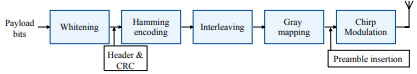
\includegraphics[scale=1]{../images/physical_lora_rx.PNG}
\caption{Etapes de la transformation des données dans un éméteur LoRa}\label{term4}
\end{figure}


Les étapes de la conception de l'envoie de données dans la couche physique de LoRa sont les suivantes :

\vspace{0.1cm}

\begin{itemize}
\item Le codage de canal est une technique utilisée dans les systèmes de communication sans fil pour améliorer la robustesse et la fiabilité de la transmission des données. Dans le cas de LoRa, le codage de canal utilise la méthode $FEC$ ($Forward$ $error$ $correction$) pour corriger les erreurs causées par du bruit. La méthode FEC ajoute de l'information redondante sur les données.
\item Le mélange de canal (ou $channel$ $interleaving$) suit la codage de canal.  
Cette technique consiste à réarranger les bits de data avant de les transmettre, en les intercalant entre eux de manière à les disperser sur le spectre des fréquences de la transmission. Cela permet de réduire l'impact des erreurs consécutives ($burst$ $error$).
\item Le blanchiment de canal (ou $channel$ $whitening$) est la dernière étape avant la modulation du signal.
Cette technique consiste à utiliser une transformation aléatoire ou pseudo-aléatoire des données avant de les transmettre, de manière à répartir le spectre des fréquences de la transmission sur une large gamme de fréquences. Cela permet également la récupération d'horloge pour le récepteur.
\item La modulation CSS est l'étape principale de LoRa. En effet, les étapes précédantes sont communes à de nombreuses technologies, mais la particularité de LoRa provient de la modulation. Cette étape est détaillée dans la section suivante du chapitre.
\end{itemize}

\vspace{0.1cm}

Chacune des étapes décrites doit être inversément réalisée pour le récepteur. Ainsi pour la récupération de donnée à l'arrivée, l'appareil récepteur gère la démodulation, le déblanchiment, le démellement et de décodage.

\vspace{0.1cm}

Cette analyse a été faite en $reverse$ $engeneering$ (\textcolor{red}{citer article}). Le reverse engineering consiste à analyser un produit ou un système afin de comprendre comment il fonctionne ou d'identifier ses principes de conception. Dans le contexte de LoRa, le reverse engineering examine la technologie derrière LoRa afin de comprendre ses principes de base et sa conception.


\subsubsection{Modulation CSS}

Contrairement aux modulation classique en amplitude ou en fréquence, la modulation CSS étale le signal sur une large bande de fréquence. La modulation en fréquence est linéaire et utilise des chirps. un chirp est un signal dont la fréquence change en continue tout en conservant une amlitude constante. Il existe deux types de chirps : les $upchirp$ et $downchirp$.
Dans un upchirp la fréquence augmente avec le temps tandis que dans un downchirp la fréquence diminue.

\vspace{0.1cm}

le signal est donc séparé sur une large bande de fréquence, permettant par exmeple plusieurs transmission sans causer d'interférence.
La modulation CSS est l'une des principale contribution au fait que LoRa possède une faible consommation et une longue portée. Cette technioque est très bien intégrée aux appareils a faible puissance utilisé par les technologies LoRa.

\subsubsection{Spreading factor}

LoRa permet d'envoyer des paquets sur un longue distance à faible puissance. Selon l'environement dans lequel les appareils LoRa sont présents, il peut être utile de pouvoir ajuster certaines capacités.

\vspace{0.1cm}

L'étalement, ou $spreading$ $factor$ permet de déterminer le taux de variation de fréquence pour un signal. Modifier le spreading factor ajuste différentes propriétés de la communications. Par exemple, si on augmente le spreading factor, les quatre conséquences principales sont :

\vspace{0.1cm}

\begin{itemize}
\item l'augmentation de la portée. Comme la largeur de bande est plus large, la communication peut atteindre une portée supérieure.
\item Augmentation de la résistance aux interférences. Comme le signal est étalé sur une bande plus largeur, il y a moins de risque de subit des interférences.
\item Plus petit débit de données. Comme la bande est large, dans un temps défini moins de données sont transmises.
\item Plus faible consommation. Les données transmises à un taux plus faible consomment moins d'énergie, ce qui prolonge la durée de vie des appareils dont l'économie d'énergie est une priorité.
\end{itemize}

Diminuer le spreading factor engendre l'effet inverse.

\subsubsection{Structure d'un paquet LoRa}

un paquet LoRa est structuré en 5 parties différentes :

\begin{itemize}
\item Le préambule : la première partie du paquet, composée d'un nombre variable d'upchirps. La valeur par défaut est fixée à 8 upchirps.
\item L'identificateur réseau : après le préambule, le paquet contient deux symbole modulé pour l'indentification réseau.
\item Des symboles de synchronization de fréquence. Après l'identificateur réseau, il y a des downchirps pour faire la dinstinction entre les offsets d'échantillionage de temps ou de fréquence.
\item La tête ($header$) du paquet. Elle contient les informations relatives à la taille du paquet, le code rate, la présence ou non d'un CRC ($cyclique$ $redundancy$ $check$) et une checksum.
\item Le payload. La dernière partie du paquet contient le payload d'une taille maximale de 255 bits et l'éventuelle CRC de 16 bits.
\end{itemize}




\subsection{LoRaWAN}

LoRaWAN est un protocol de type $low$ $power$, $wide$ $area$ $network$ (LPWAN) désigné pour la communication longue portée. Ce protocole opère avec la technologie LoRa et lui fournit une infrastructure capable de maintenir une communication à longue portée et à faible cout dans l'$IoT$.

\textcolor{red}{FIN REDACTION}

\subsubsection{avantage}

pourquoi s'en servir ?,
faible puissance, 
portée accrue, 
pénétration efficace de l'environement,
déploiment ne nécessite pas de license,
géolocalisable (le réseau peut détecter les devices),
réseau public et privé,
sécurité en end to end,
mise à jour des micrologicielle par les air,
programme de certification,
vaste ecosystème,

\subsubsection{use case}

use case:
aspect environemental 
catastophe naturelle prevention,
agriculture intelligente et supervision animale,
protection des expèces menacées

axpect inductrielle
controle smart cities
approvisionnement chaine logistique
gestion installations diverses

\subsubsection{limitations}

payload limité (entre 51 et 241 octets)

data rate faible (maximum 5.5 kbps sur une bande de 125Hz)

restrictions liées aux régions (US, EU)

communication asynchrone 


\subsubsection{topologie}

\textcolor{red}{image network lorawan}

lora devices et lora gateway. gateway écoute plusieurs fréquence simultanément (multichanneling) tant qu'un end devices écoute une seule fréquence à la fois. transport entre end devices et gateway : uplink. sens inverse downlink.


end nodes connecté a des gateway. pas de lien direct le gateway écoute les end devices. les gateway forward les message jusqu'à un server réseau. les serveur indentifie le end devices. il gère la partie sécurité, l'information arrive à l'application.

LoRaWAN peut adapter le data rate en focntion de la topologie. par exemple ajuster le spreading factor en fonction de la distance entre les devices et les gateway. (ex : longue distance = grand spreading factor, lower data rate)

possibilité de mesurer la qualité du canal de communication (SNR). ex ajuster le datarate si bcp de bruit

Device class :
A end nodes (most common), 
B beacon (deep sleep),
C continuous downlink.

\subsubsection{securité}

Autentification : qui communique avec qui

intégrité : les données ne sont pas altéré entre émteur et récepteur

confidentialité : le réseau ne peut pas voir les données.

chiffrage en AES
deux types de clefs

$root$ $key$ : clé partagé entre un end device et le serveur réseau. Utilisée pour l'authentification initiale et l'établissement d'une communication entre les deux éléments du réseau. Cette clé n'est jamais transmise par els air et est stockée dans un $join$ $server$

$session$ $keys$ : clé générée dynamiquement et utilisé durant l'échnage de donnée pendant une session. Il y a deux session key différente, la AppSKEY pour le chiffrage des payload d'application, et la nwkSKEY pour les fonctionalité du réseau (chifrage à la couche MAC, integrity checks, etc).

un join server est un server dédié au contenu sensible à l'activation du matériel dans un réseau LoRaWAN. Il autentifie le réseau et les aplication du servers. Il gère les $root$ $keys$. il génère les $session$ $keys$ et les distribue.

Taille de clé de 128 bits,.
pk aes et cette taille de clés ? pas trop de ressources donc taille minimale standard en terme de sécurité

\subsubsection{session}

deux types de sessions :

1 network session:

adresse du devices, la session key, MAC state et frame counters

2 application session:

la session key, frame counters

la $frame$ $counter$ est une stratégie de défense servant à éviter les $replay$ $attacks$, en rejttant les données dépassée ou retransmise. 


comment établir une session ?

de manière dynamique en rejoigant un réseau (Over the air Activation $OTAA$) ou hardcodé (activation personalisée $ABP$)
OTAA:
procedure entre end devices et serveur réseau
les clés sont regénérées à chaque nouvelle session
ABP (moins safe mais moins contraignant en terme de ressources):
pas de procédure
les clés sont hardcodés
